\chapter{Entwicklung einer real-time Query Anwendung zur Beschleunigung von Userprofilqueries}
Ein wesentlicher Bestandteil der bestehenden Betriebsanwendung bildet das Abfragen von Userprofildaten. Um für Umfragen passgenau Teilnehmer auszuwählen, gibt es in der Profildatenbank, die knapp 400.000 Nutzer umfasst, 176 Profilfelder. Diese können in allen denkbaren Kombinationen abgefragt werden. Die besteheden Datenbankabfragen geschehen aufgrund ihrer langen Laufzeit asynchron. Hier soll eine neue, synchrone Schnittstelle geschaffen werden.

\section{Real-time Anforderungen erzwingen eine neue Entwicklung}
Da das Finden von Umfrageteilnehmern und demnach das Abfragen der Profilfelder einen wesentlichen Kern der Betriebsanwendung bildet, besteht dieser Teil der Anwendung mit am längsten. In den fast 3 1/2 Jahren ist sowohl die Anzahl der User, also auch die Anzahl der Profilfelder enorm gewachsen, weitaus mehr als initial erwartet. Im Laufe der Zeit stellte sich heraus, das die gewählte Datenbanktechnologie MongoDB, das gewählte ``Schema'' (FIX NO SCHEMA!) und die Art wie gequeried wird, nicht optimal und daher nicht schnell genug sind. Da das Abfragen der Profilfelder wesentlichster Bestandteil des Kerngeschäfts ist und die Defizite die Situation mit wachsender User- und Kundenzahl nur verschärfen, wurde deutlich, dass eine Überarbeitung der bestehenden Strukturen notwendig ist.

\section{Majestic Monolith vs Minimal Microservice}
Um die Probleme zu lösen kann auf vielerlei Wege vorgegangen werden. Eine neue Datenbanktechnologie mit optimiertem Schema kann gewählt werden, der Code kann auf Geschwindigkeit optimiert oder komplett neu geschrieben werden.
Die hier eingesetzte Datenbank MongoDB wird noch für weitere Funktionen in der Anwendung genutzt und kann daher nicht komplett ersetzt werden. Eine bestehende MySQL Datenbank ist bereits als Datawarehouse im Einsatz und erfährt bereits load.
Die bestehende Anwendung ist mit den Jahren allgemein recht groß und unhandlich geworden.
Eine Aufsplittung der Anwenung in mehrere Teile, mit Hilfe der Microservice Architektur, wurde beschlossen.
Mit Hilfe der Microservice Architektur können hier Probleme der Skalierung, Optimierung der Datenbanktechnologie, Beschleunigung des Codes und Schaffung von Ordnung im Code angegangen werden.
Da eine neue Datenbanktechnologie und ein komplett separater Service ohnehin mit vielen Änderungen verbunden ist, wurde beschlossen den alten Code nicht in einen neuen Service zu migrieren, sondern die Funktionalität neu zu Schaffen.

\section{Mit dem Strangler Pattern vom Monolithen zur Microservice Architektur}
Da die aktuelle Arbeitslage, die vorhandenen Entwickler und die Größe der Anwendung es nicht zulassen diese direkt komplett zu überarbeiten, wird hier die Architektur mit Hilfe des Strangler Patterns~\footcite[][]{Fowler:Strangler} Schritt für Schritt umgesetzt.
Der Name des Stangler Patterns ist aus einer Analogie zur Botanik entstanden. Hierbei wurde von Fowler der Vergleich zur Würgefeige (engl. Strangler Fig) gezogen. Diese wächst von den Ästen an einem Wirtsbaum herab, bis sie den Boden erreicht. Nach und nach wird der Wirtsbaum immer weiter umschlossen, bis er schließlich abstirbt.
Ähnlich kann bei der Softwareentwicklung zum Ersetzen einer alten Anwendung vorgegangen werden. An bestimmten, sich eignenden Stellen wird begonnen Teile der bestehenden Anwendung zu ersetzen. Neuer Code wird geschaffen und nach und nach die Last auf die neue Teilanwendung geleitet.
Dieses Vorgehen bietet viele Vorteile gegenüber dem kompletten Austausch einer Altanwendung. Die neue Anwendung kann Stück für Stück mit agilen Methoden und häufigen deploys entwickelt und im Produktionsbetrieb betrachtet werden. Die neu entstehende Anwendung kann hierbei nach Belieben angepasst werden, um die Altanwendung am problemlosesten zu Ersetzen.
Zur Umsetzung dieses Ersetzens gibt es viele Wege. Zwei ebenfalls von Fowler vorgebrachte Strategien sind AssesCapture~\footcite[][]{Fowler:Capture} und EventInterception~\footcite[][]{Fowler:Interception}.
Beim AssetCapture geht es vor Allem darum, Assets zu identifizieren, die sich leicht in die neue Teilanwendung migrieren lassen. Dies können bestimmte Tabellen in der Datenbank sein. Im Fall der zu entwickelnden Anwendung sind dies die Userprofile.
EventInterception geht mit AssetCapture Hand in Hand. Hierbei müssen alle Events auf die ausgelagerten Assets, also zum Beispiel das Abfragen von Profilen und das Anlegen neuer Profile, abgefangen und umgeleitet werden.
So wird sichergestellt, dass die alten Ressourcen nicht mehr aktualisiert werden und es nicht zu Inkonsitenzen im Datenbestand kommt,
Um die bestehende Betriebsanwendung auf Microservices umzustellen, wird hier ähnlich vorgegangen. Aus gegebenem Anlass wird der Query-Microservice als erster Strangler entwickelt. Die Userprofile eignen sich gut um sie in eine neue Datenbank zu migrieren und in diesem Schritt gleeich zu optimieren. Ein neuer Service verwaltet hierzu den Zugriff auf die Daten. Die bestehenden Events zum Abfragen von Userprofildaten werden auf den neuen Service umgestellt. Hier wird eine Schnittstelle geschaffen, die sowohl Zugriff auf den neuen Service, als auch auf die alte Datenbank zulässt.
\begin{figure}[h]
    \caption{Load Balancer zur Strangulation Verteilung (~\cite{Hammant:Strangler})}
    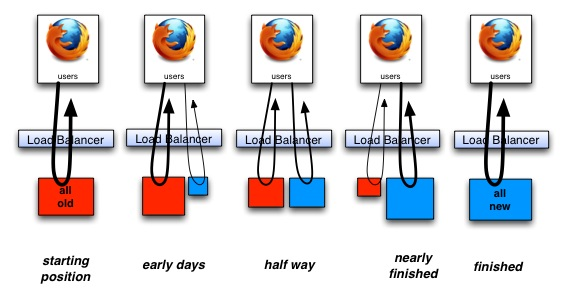
\includegraphics[width=\textwidth]{strangulation}
\end{figure}
Statt traditionellem Load Balancer, wird hier mit Hilfe des Ruby Flipper Gems~\footnote{https://github.com/jnunemaker/flipper} nach und nach mehr Last auf den neu entstehenden Service verteilt.~\footcite[vgl.][]{Hammant:Strangler}
Da die Userprofile noch auf Seiten der Verwaltung der User selbst in der Hauptanwendung benötigt werden, werden hier jedoch nicht alle Event abgefangen. Lediglich die, die das Querien im Bereich des Samplings betreffen. Um Datenkonsitenz zu gewährleisten, werden einmal täglich alle veränderten Daten in den Microservice geupdated. Da sich Userdaten nicht häufig ändern und sich unter 100 Nutzer am Tag registrieren, reicht dies aus um ausreichend gute Query Ergebnisse zu erzielen.